% Prepared by Calvin Kent
\documentclass[12pt,oneside]{book} %
\usepackage{CKpreamble}
\usepackage{CKlecture}
\usepackage{mdframed}
\usepackage{import}
\usepackage{pdfpages}
\usepackage{euscript}
\usepackage{transparent}
\usepackage{xcolor}
\usepackage{tasks}
\usepackage{physics}
\usepackage{tkz-euclide}


%%% Maths and science packages

\def\aehlength{3}

\usepackage{amsmath,amsthm,amssymb}
\usepackage{pgfplots}
	\usetikzlibrary{
		calc,
		patterns,
		positioning
	}
	\pgfplotsset{
		compat=1.16,
		samples=200,
		clip=false,
		my axis style/.style={
			axis x line=middle,
			axis y line=middle,
			legend pos=outer north east,
			axis line style={
				->,
			},
			legend style={
				font=\footnotesize
			},
			label style={
				font=\footnotesize
			},
			tick label style={
				font=\footnotesize
			},
			xlabel style={
				at={
					(ticklabel* cs:1)
				},
				anchor=west,
				font=\footnotesize,
			},
			ylabel style={
				at={
					(ticklabel* cs:1)
				},
				anchor=west,
				font=\footnotesize,
			},
			xlabel= $x$,
			ylabel=$\vec d (\m \tx{[East]})$
		},
	}
	\tikzset{
		>=stealth
	}

\pgfplotsset{my style/.append style={axis x line=middle, axis y line=
middle, xlabel={$x$}, ylabel={$y$}, axis equal }}

\newcommand{\incfig}[2][1]{%
    \def\svgwidth{#1\columnwidth}
    \import{./figures/}{#2.pdf_tex}
}


\newcounter{step}[section]
\newenvironment{step}[1][]
{\refstepcounter{step} \textit{Step #1.}}

\newcounter{Rule}[section]
\newenvironment{Rule}[1][]
{\refstepcounter{Rule} \textit{Rule #1.}}


\pdfsuppresswarningpagegroup=1

%
\renewcommand*{\doctitle}{Class Based Lecture Notes}
\makeatletter\patchcmd{\chapter}{\if@openright\cleardoublepage\else\clearpage\fi}{}{}{}\makeatother % only used in class based
\begin{document}
	% Start of Class settings
	\renewcommand*{\term}{Term 2} % Term
	\renewcommand*{\coursecode}{MCR3U} % Course code
	\renewcommand*{\coursename}{Course Name} % Full course name
	\renewcommand*{\thelecnum}{9} % Lecture number
	\renewcommand*{\profname}{Prof Name} % Prof Name
	\renewcommand*{\colink}{http://www.student.math.uwaterloo.ca/~c2kent} % Course outline link
	% End of Class settings
	\clearpage
	\pagenumbering{arabic}
	\pagestyle{classlecture}
	%%% Note to user: CTRL + F <CHANGE ME:> (without the angular brackets) in CKpreamble to specify graphics paths accordingly.
	%%% If a new chapter was started in the middle of a lecture, \fix chap{Second Chapter} must be used immediately above the next lecture.
	% Course notes start
\setchap{9}{Trigonometry Part II}
\begin{lec}{January 2022}
	\chapter{\chapname\chaplec}

  \section{Motivation}
  Recall the equation of a circle with radius $r$,
  \[
      x^2 + y^2 = r^2
  \] 

   \begin{center}
    \begin{tikzpicture}
      \begin{axis}[
          my style,
          ytick=\empty,
          xtick=\empty,
          xticklabels=\empty,
          yticklabels=\empty,
        ]

        \draw (axis cs: 0, 0) circle [radius=2];% I've set the radius to 10 only for better show the image
        \draw (45:2) node[circle,fill,draw,inner sep=2pt] {};
        \draw (45:2) node[right,circle,inner sep=2pt]{$\textbf{P}(x,y)$};

        \addplot[domain=-2.5:2.5, white]{-x};


      \end{axis}
    \end{tikzpicture}
   \end{center}
   
   We would like a more efficient way of determining coordinates $\textbf{P}(x,y)$ around the circle. To do so we employ
   some trigonometry to therefore introduce a different way to so called $ \textit{parametrize}$ the circle. By
   $\textit{parametrize}$ we mean to define a new metric for measuring coordinates in standard euclidean geometry.
   You'll see why this ends up being more efficient.

   \section{Introduction}

   \begin{defn}
       Given a circle, the \textbf{terminal arm} at a point $\textbf{P}$ is a ray from the origin to the point $\vb P$.
   \end{defn}

   \begin{ex}
     Suppose we have a circle $x^2 + y^2 = 4$ and points $\vb P, \vb R, \vb Q$. The following is a diagram of their
     corresponding terminal arms,

         \begin{center}
          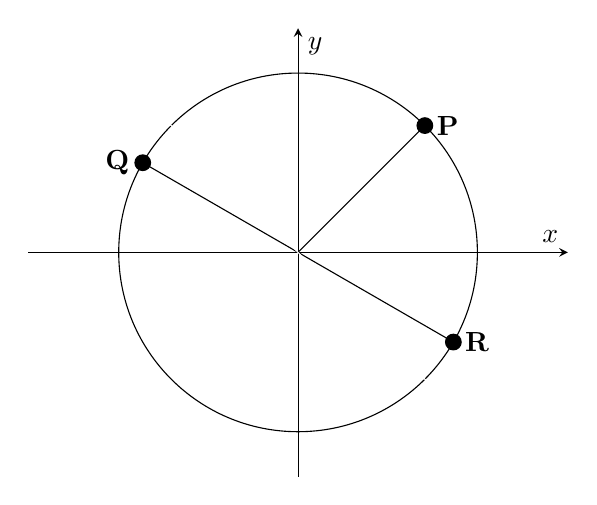
\begin{tikzpicture}
            \begin{axis}[
                my style,
                ytick=\empty,
                xtick=\empty,
                xticklabels=\empty,
                yticklabels=\empty,
              ]

              \draw (axis cs: 0, 0) circle [radius=2];% I've set the radius to 10 only for better show the image

              \draw (0,0) -- (45:2) node[midway, above] {};
              \draw (0,0) -- (150:2) node[midway, above] {};
              \draw (0,0) -- (330:2) node[midway, above] {};

              \draw (45:2) node[circle,fill,draw,inner sep=2pt] {};
              \draw (150:2) node[circle,fill,draw,inner sep=2pt] {};
              \draw (330:2) node[circle,fill,draw,inner sep=2pt] {};

              \draw (45:2) node[right,circle,inner sep=2pt]{$\vb P$};
              \draw (150:2) node[left,circle,inner sep=2pt]{$\vb Q$};
              \draw (330:2) node[right,circle,inner sep=2pt]{$\vb R$};

              \addplot[domain=-2.5:2.5, white]{-x};


            \end{axis}
          \end{tikzpicture}
         \end{center}
   \end{ex}

   \begin{defn}
       \textbf{Polar coordinates} are a metric defined on circles where each coordinate is defined as
       $\vb P(r,\theta)$. Here, $r$ corresponds to the radius of the circle and $\theta$ corresponds to the angle of the
       terminal arm at $\vb P$, known as the terminal angle.
   \end{defn}

   \begin{ex}
     Given a circle $x^2 + y^2 = 9$, plot the following polar coordinates,
     \begin{enumerate}[label=(\alph*)]
       \item $\vb P(3, 60^{\circ})$
       \item $\vb Q(3, 120^{\circ})$ \hfill (**)
       \item $\vb R(3, 240^{\circ})$
       \item $\vb T(3, 330^{\circ})$ \hfill (**)
     \end{enumerate}

   \end{ex}

   \subsection*{Negative angles}
   \begin{rem}
       Given a polar coordinate $\vb P(r, \theta)$, if  $\theta > 0^{\circ}$ then this corresponds to a counter-clockwise rotation
       of our terminal arm to pivot it to its correct position on the circle. However if $\theta < 0^{\circ}$, then we
       rotate clockwise.
   \end{rem}

   \begin{ex}
     Given a circle $x^2 + y^2 = 4$, plot the following polar coordinates,
     \begin{enumerate}[label=(\alph*)]
       \item $\vb P(2, 60^{\circ})$
       \item $\vb Q(2, -330^{\circ})$
       \item $\vb K(2, -240^{\circ})$ \hfill (**)
       \item $\vb N(2, -40^{\circ})$ \hfill (**)
     \end{enumerate}

   \end{ex}

   \subsection*{Reference angles}
   \begin{defn}
     Given a polar coordinate $\vb P(r, \theta)$, the \textbf{reference angle} $\alpha$ is the \underline{acute angle} between the
     terminal arm at $\vb P$ and the x-axis.
   \end{defn}

   \begin{ex}
     Given a circle $x^2 + y^2 = 4$, for each of the following polar coordinates determine the corresponding
     reference angle,
    \begin{tasks}(6)
       \task $\vb P(2, 60^{\circ})$
       \task $\vb R(2, 150^{\circ})$
       \task $\vb Q(2, 180^{\circ})$ \, (**)
       \task $\vb T(2, 240^{\circ})$ \, (**)
       \task $\vb G(2, 270^{\circ})$
       \task $\vb H(2, 340^{\circ})$ \, (**)
    \end{tasks}

   \end{ex}

   \begin{ex}[Negative Angles]
     Given a circle $x^2 + y^2 = 4$, for each of the following polar coordinates determine the corresponding
     reference angle,
    \begin{tasks}(5)
       \task $\vb P(2, -45^{\circ})$
       \task $\vb R(2, -90^{\circ})$
       \task $\vb Q(2, -120^{\circ})$ \, (**)
       \task $\vb T(2, -230^{\circ})$ \, (**)
       \task $\vb G(2, -330^{\circ})$ \, (**)
    \end{tasks}

   \end{ex}

   \newpage

   \begin{thrm}[CAST Rule]
     Given a polar coordinate $\vb P(r,\theta)$,
     \begin{itemize}
       \item If the terminal arm lies in quadrants  I or IV, then $\cos \theta$ is positive.
       \item If the terminal arm lies in quadrants  I or II, then $\sin \theta$ is positive .
       \item If the terminal arm lies in quadrants  I or III, then $\tan \theta$ is positive.
     \end{itemize}
     This can be summarized into the so called CAST rule,

         \begin{center}
          \begin{tikzpicture}
            \begin{axis}[
                my style,
                ytick=\empty,
                xtick=\empty,
                xticklabels=\empty,
                yticklabels=\empty,
              ]

              \draw (45:2) node[right,circle,inner sep=2pt]{\textbf{A}ll};
              \draw (135:2) node[right,circle,inner sep=2pt]{\textbf{S}ine};
              \draw (225:2) node[right,circle,inner sep=2pt]{\textbf{T}an};
              \draw (315:2) node[right,circle,inner sep=2pt]{\textbf{C}osine};

              \addplot[domain=-2.5:2.5, white]{-x};


            \end{axis}
          \end{tikzpicture}
         \end{center}
     
   \end{thrm}

   \begin{thrm}[Angle Symmetry]
     Given an angle $\theta$, the following symmetric relationship holds
    \[
        \cos \theta = \pm \cos \alpha \hspace*{1.1cm} \sin \theta = \pm \sin \alpha
                                \hspace*{1.1cm} \tan \theta = \pm \tan \alpha
   .\] Where,
   \begin{itemize}
     \item $\alpha$ is the corresponding reference angle.
     \item The $(\pm)$ sign can be determined by using the CAST rule.
   \end{itemize}
   \end{thrm}

   \begin{ex}
     Determine the exact value of the following trigonometric ratios,
          \begin{tasks}(5)
             \task $\sin 60^{\circ}$
             \task $\cos 120^{\circ}$ 
             \task $\tan 210^{\circ}$ 
             \task $\sin 270^{\circ}$ 
             \task $\cos 300^{\circ}$ 
          \end{tasks}
   \end{ex}

   \section{Converting :  $\vb P(r, \theta) \rightarrow \vb P(x,y)$}

   \begin{thrm}
     Given a polar coordinate $\vb P(r, \theta)$, the corresponding standard coordinates are,
    \[
        x = r\cos \theta \hspace*{1cm} y = r\sin \theta
   .\]
   \end{thrm}


   \begin{ex}
     Convert the following polar coordinates to standard coordinates,
    \begin{tasks}(5)
       \task $\vb P(2, 60^{\circ})$
       \task $\vb Q(2, 120^{\circ})$ \\ (**)
       \task $\vb T(4, 210^{\circ})$ \\ (**)
       \task $\vb M(1, 270^{\circ})$ 
       \task $\vb G(6, 330^{\circ})$ \\ (**)
    \end{tasks}
   \end{ex}

   \newpage

   \begin{ex}[Negative Angles]
     Convert the following polar coordinates to standard coordinates,
    \begin{tasks}(5)
       \task $\vb P(2, -45^{\circ})$
       \task $\vb R(3, -180^{\circ})$
       \task $\vb Q(4, -150^{\circ})$ \, (**)
       \task $\vb G(8, -300^{\circ})$ \, (**)
    \end{tasks}
    \end{ex}

    \section{Solving Trigonometric equations}
    Suppose we were given one of the following trigonometric ratios where the angle $\theta$ is unknown,
    \[
        \cos \theta = \frac{x}{r} \hspace*{1.1cm} \sin \theta = \frac{y}{r}
                                \hspace*{1.1cm} \tan \theta = \frac{y}{x}
   .\]
   Suppose that we know the quadrant in which the angle $\theta$ lies within, then we can use the following
   procedure to solve for $\theta$,

    \begin{step}[1]
      Draw the terminal arm corresponding to the quadrant in which $\theta$ lies within.
    \end{step}
     
    \begin{step}[2]
      Compute the reference angle $\alpha$,
    \[
        \alpha = \cos^{-1}\left( \left|\frac{x}{r}\right|\right)  \hspace*{1.1cm}
        \alpha = \sin^{-1}\left( \left|\frac{y}{r}\right|\right) \hspace*{1.1cm}
        \alpha = \tan^{-1}\left( \left|\frac{y}{x}\right|\right)
   .\]
    \end{step}
    
    \begin{step}[3]
      Use $\alpha$ as well as your diagram to compute $\theta$.
    \end{step}

    \begin{ex}
      For each of the following, you are given a trigonometric ratio, solve for $\theta$. 
      Assume that each angle  $\theta$ lies in the \textbf{third} quadrant.
        \begin{tasks}(3)
           \task $\cos \theta_1 = -\frac{1}{2}$
           \task $\sin \theta_2 = -\frac{\sqrt{3}}{2} $ \\ (**)
           \task $\tan \theta_3 = 1 $ \\ (**)
        \end{tasks}
    \end{ex}

    \begin{ex}
      For each of the following, you are given a trigonometric ratio, solve for $\theta$. 
      Assume that each angle  $\theta$ lies in the \textbf{second} quadrant.
        \begin{tasks}(2)
           \task $\cos \theta_1 = -\frac{1}{4}$
           \task $\sin \theta_2 = \frac{1}{\sqrt{2}} $ \\ (**)
        \end{tasks}
    \end{ex}

   \section{Converting :  $\vb P(x,y) \rightarrow \vb P(r, \theta)$}

   \begin{thrm}
     Given standard coordinates $\vb P(x,y)$, the corresponding polar coordinates are,
    \[
        r = \sqrt{x^2 + y^2} \hspace*{1.2cm} \tan \theta = \frac{y}{x}
   .\]
   Where $\theta$ is the solution to the trigonometric equation.
   \end{thrm}

   \begin{ex}
     Convert the following standard coordinates to polar coordinates,
    \begin{tasks}(4)
       \task $\vb P\left(2, 2\sqrt{3}\right)$
       \task $\vb Q(2, -5)$
       \task $\vb T\left(-6,-8 \right)$ \\ (**)
       \task $\vb M\left(-3\sqrt{3}, 3\right)$ \\ (**)
    \end{tasks}
   \end{ex}


  

	\end{lec}

\end{document}




















 































